The \textit{User Management} module is responsible for maintaining demographic information
about the registered users of the system, including the Authority levels of each
user.

\subsection{Scope}
The scope for the users module is shown in Figure \ref{Users Scope}
\begin{figure}[H]
  \begin{center}
  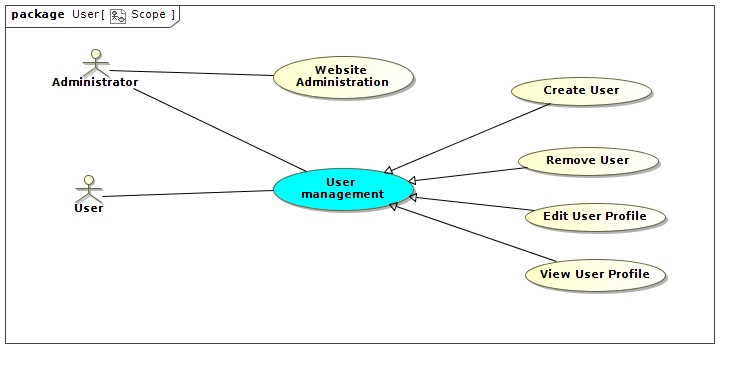
\includegraphics[scale=0.5]{../Diagrams and Charts/Users/Scope.jpg}
  \caption{Users Scope}
  \end{center}
  \label{Users Scope}
\end{figure}
The scope of the users module include:
\begin{itemize}
	\item The Super User can add and remove Administrator users
	\item Administrator users can add and remove Regular Users
	\item Any person who wants use the benchmarking service can register
	to the system and become a user. They can then also edit
	their profile or de-register.
	\item Any user can view the profile of any Administrator or Regular
	user.
\end{itemize}

\subsection{Domain Model}
The domain model for the users module is shown in Figure \ref{Users Domain Model}
\begin{figure}[H]
  \begin{center}
  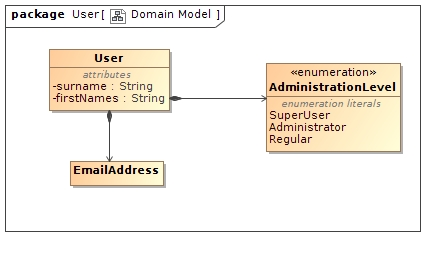
\includegraphics[scale=1.0]{../Diagrams and Charts/Users/Domain Model.jpg}
  \caption{Users Domain Model}
  \end{center}
  \label{Users Domain Model}
\end{figure}
For each user a Surname, First Names and Email Address will be stored.
There are 3 main types of users who
are at different authority levels. There is one and only one "Super User" who
will have full authority over the entire system. Then there are "Administrator"
users who can be assigned or removed by the Super User. The main function of
the Super User is to manage the Administrator users. The Administrator user
will have the permissions needed to manage the website and to add or remove
regular users if necessary. Lastly the "Regular Users"
can be registered by anyone who wants to use the benchmarking service. These users
will be able to use the service but not do anything administrative.

\subsection{Change Password}
Changes the associated password with the current logged in user.

\subsubsection{Services Contract}
Figure \ref{fig:changePasswordServicesContract} depicts the service contract for the \textbf{changePassword} service.

\begin{figure}[H]
  \begin{center}
  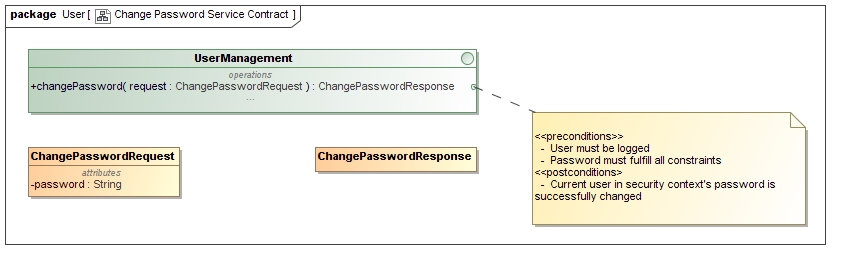
\includegraphics[scale=0.55]{../Diagrams and Charts/Users/Change Password Service Contract.jpg}
  \caption{Service contract for the changePassword use case}
  \label{fig:changePasswordServicesContract}
  \end{center}
\end{figure}

For a user to change their associated password the following must hold true:
\begin{itemize}
	\item The user must be logged in.
	\item The user must exist in the current security context
	\item The new password must subscribed to all validation requirements.
\end{itemize}

If the user is not logged in, a \textbf{NotAuthorized} exception is thrown.

If the user doesn't exist in the current security context, a \textbf{NonExistentException} is thrown.

If the password doesn't fulfill the required validation requirements, a \textbf{validationException} is thrown.

In addition, the service will be refused if the request does not comply to the data structure specification.

\subsubsection{Functional Requirements}
Figure \ref{fig:changePasswordUseCase} shows the lower level services required by the changePassword service.

\begin{figure}[H]
	\begin{center}
		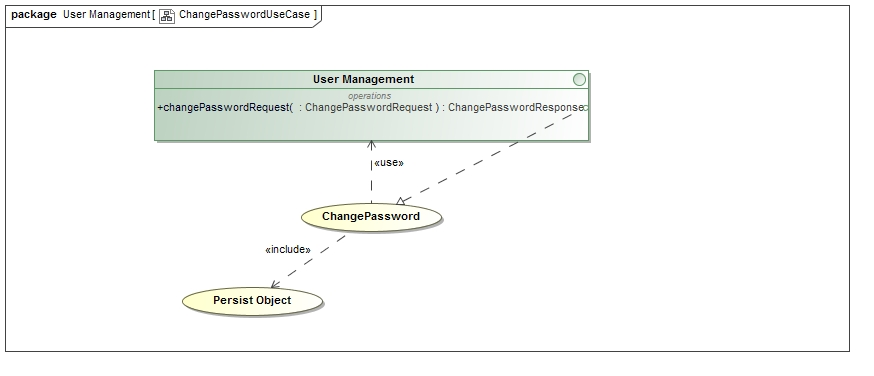
\includegraphics[scale=0.55]{../Diagrams and Charts/Users/Change Password Use Case.jpg}
		\caption{Service contract for the changePassword use case}
		\label{fig:changePasswordUseCase}
	\end{center}
\end{figure}
\subsubsection{Process design}

\subsection{Complete Password Reset}
Completes the password reset of a user who us currently resetting their password.

\subsubsection{Services Contract}
Figure \ref{fig:completePasswordResetServicesContract} depicts the service contract for the \textbf{completePasswordReset} service.

\begin{figure}[H]
  \begin{center}
  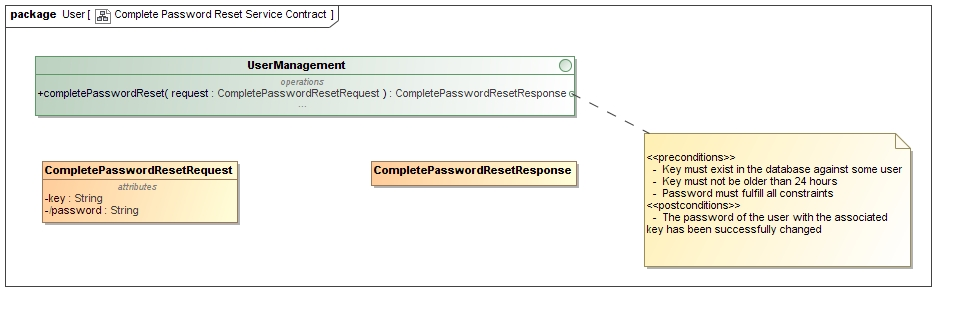
\includegraphics[scale=0.55]{../Diagrams and Charts/Users/Complete Password Reset Service Contract.jpg}
  \caption{Service contract for the completePasswordReset use case}
  \label{fig:completePasswordResetServicesContract}
  \end{center}  
\end{figure}

For a user to complete the reset of their password the following must hold true:
\begin{itemize}
	\item The associated key must be linked to a user object.
	\item The key must not be older than 24 hours
	\item The new password must subscribed to all validation requirements.
\end{itemize}

If the key is not associated with a user or the key is older than 24 hours a \textbf{NotAuthorized} exception is thrown.

If the password doesn't fulfill the required validaiton requirements, a \textbf{Validation} exception is thrown.

In addition, the service will be refused if the request does not comply to the data structure specification.

\subsubsection{Functional Requirements}
Figure \ref{fig:completePasswordResetFunctionalRequirements} shows the lower
level services required by the completePasswordReset service.

\begin{figure}[H]
	\begin{center}
		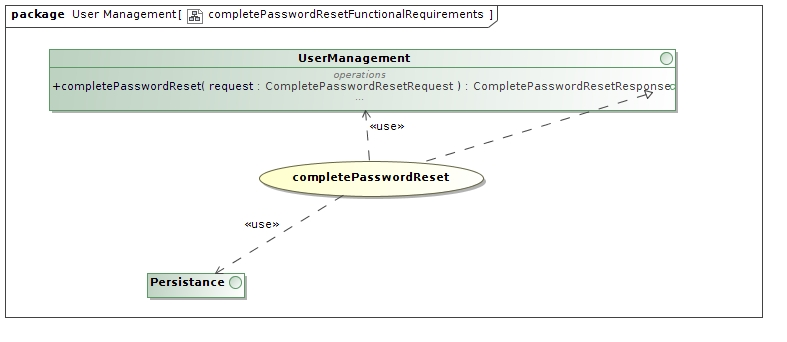
\includegraphics[scale=0.55]{../Diagrams and Charts/Users/completePasswordResetFunctionalRequirements.jpg}
		\caption{Functional Requirements for the completePasswordReset use case}
		\label{fig:completePasswordResetFunctionalRequirements}
	\end{center}
\end{figure}

The only real lower level requirement is that a persistance interface is requiered
to access the database.

\subsubsection{Process design}

\subsection{Request Password Reset}
Starts the process to allow a user to reset their password.

\subsubsection{Services Contract}
Figure \ref{fig:requestPasswordResetServicesContract} depicts the service contract for the \textbf{requestPasswordReset} service.

\begin{figure}[H]
  \begin{center}
  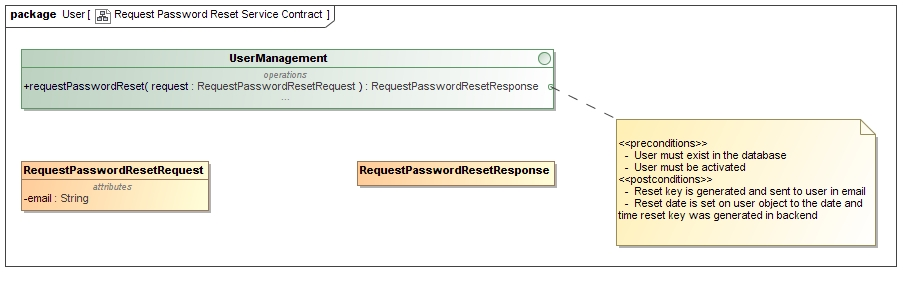
\includegraphics[scale=0.55]{../Diagrams and Charts/Users/Request Password Reset Service Contract.jpg}
  \caption{Service contract for the requestPasswordReset use case}
  \label{fig:requestPasswordResetServicesContract}
  \end{center}  
\end{figure}

For a user to request a reset of their associated password the following must hold true:
\begin{itemize}
	\item The user must be registered.
	\item The user must not have outstanding pending reset requests.
\end{itemize}

If any of the above doesn't hold, a \textbf{NotAuthorized} exception is thrown.

The following must also hold true:
\begin{itemize}
	\item The user must be activated
\end{itemize}

If any of the above doesn't hold, a \textbf{UserNotActivatedException} exception is thrown.

Futhermore the \textbf{EmailNotRegisteredException} and \textbf{EmailNotSentException}
will be thrown if either the email address in the request object does not belong
to a registered user or if the sending of the email failed for some reason.

In addition, the service will be refused if the request does not comply to the data structure specification.

\subsubsection{Functional Requirements}
Figure \ref{fig:requestPasswordResetFR} shows the lower level services required by the requestPasswordReset service.

\begin{figure}[H]
	\begin{center}
		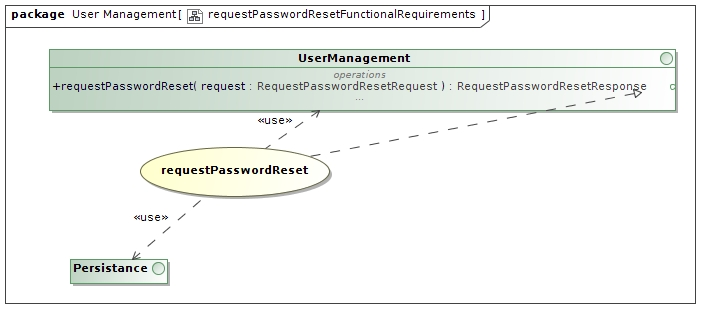
\includegraphics[scale=0.55]{../Diagrams and Charts/Users/requestPasswordResetFunctionalRequirements.jpg}
		\caption{Functional Requirements for the requestPasswordReset use case}
		\label{fig:requestPasswordResetFR}
	\end{center}
\end{figure}

The only real lower level requirement is that a persistance interface is requiered
to access the database.

\subsubsection{Process design}

\subsection{Create Managed User}
Creates a managed user.

\subsubsection{Services Contract}
Figure \ref{fig:createManagedUserServicesContract} depicts the service contract for thr \textbf{createManagedUser} service.

\begin{figure}[H]
	\begin{center}
		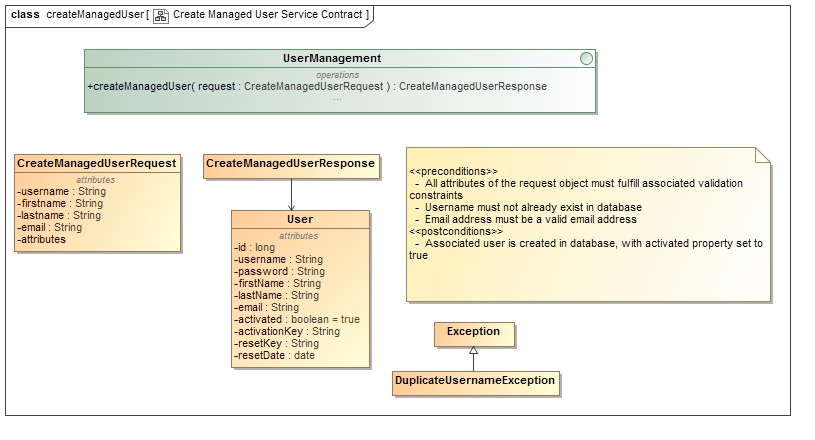
\includegraphics[scale=0.55]{../Diagrams and Charts/Users/Create Managed User Service Contract.jpg}
		\caption{Service contract for the createManagedUser use case}
		\label{fig:createManagedUserServicesContract}
	\end{center}
\end{figure}

To create a managed user the following must hold true
\begin{itemize}
	\item Attributes of the request object must fulfill validation constraints.
	\item Username cannot exist in the database.
	\item Email address must be valid.
\end{itemize}

If the username already exists in the database, a \textbf{DuplicateUsernameException} will be thrown.

If the email address provided already exists in the database, a \textbf{EmailAlreadyExistsException}
will be thrown

If the validation requirements aren't met, a \textbf{validationException} will be thrown.

\subsubsection{Functional Requirements}
Figure \ref{fig:createManagedUserUseCase} depicts the use case for the \textbf{createManagedUser} service.

\begin{figure}[H]
	\begin{center}
		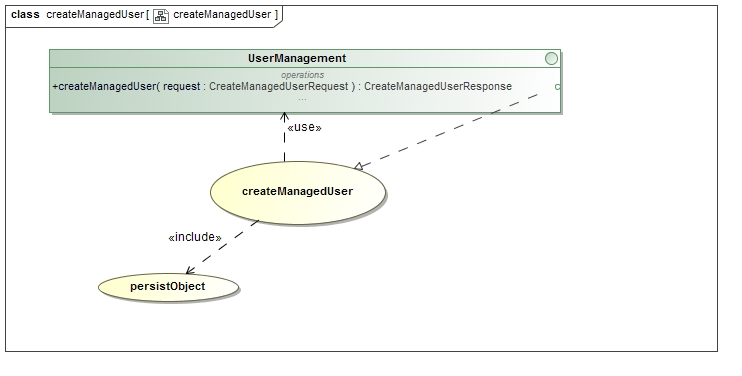
\includegraphics[scale=0.55]{../Diagrams and Charts/Users/Create Managed User Use Case.jpg}
		\caption{Use case for the createManagedUser use case}
		\label{fig:createManagedUserUseCase}
	\end{center}
\end{figure}

\subsection{Create Unmanaged User}

\subsubsection{Services Contract}
Figure \ref{fig:CreateUnmanagedUserServicesContract} depicts the service contract
for the \textbf{createUnmanagedUser} service.
Used to create a user with a user selected password and role of a normal user. 
This is used for registration on the front end of the API.

\begin{figure}[H]
  \begin{center}
  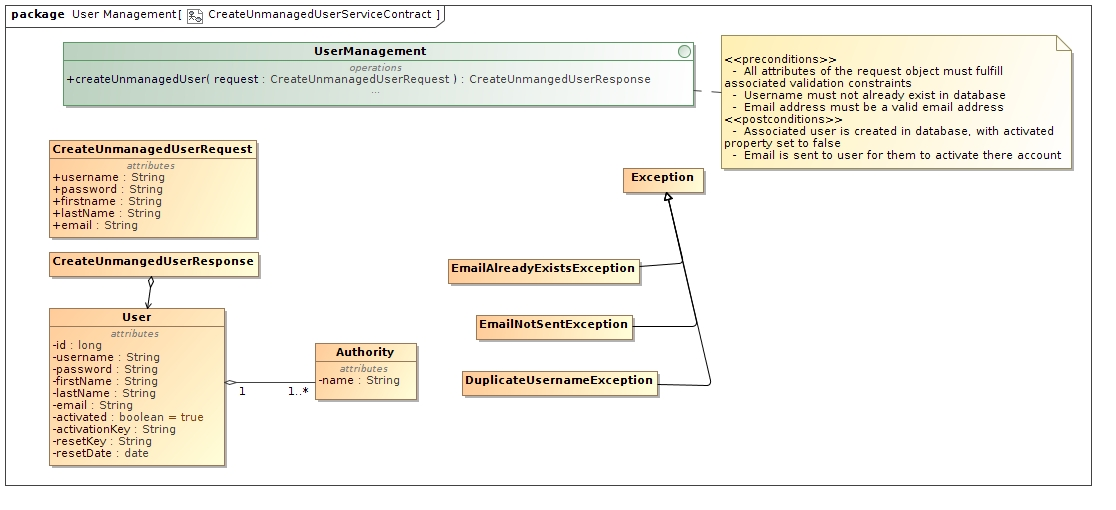
\includegraphics[scale=0.4]{../Diagrams and Charts/Users/CreateUnmanagedUserServiceContract.jpg}
  \caption{Service contract for the createUnmanagedUser use case}
  \label{fig:CreateUnmanagedUserServicesContract}
  \end{center}  
\end{figure}

For an unmanaged user to be created the following must hold.
\begin{itemize}
	\item Username must not already exist in database.\\
	Otherwise a \textbf{DuplicateUsernameException} is thrown.
	\item Email address must be a valid email address that is not already in the system.\\
	Otherwise a \textbf{EmailAlreadyExistsException} is thrown.
	\item If for some reason the email for activation could not be sent
	a \textbf{EmailNotSentException} will be thrown.
\end{itemize}

In addition, the service will be refused if the request does not comply to the data structure specification.

\subsubsection{Functional Requirements}
Figure \ref{fig:CreateUnmanagedUserFR} shows the lower level services required
by the \textbf{createUnmanagedUser} service.

\begin{figure}[H]
	\begin{center}
		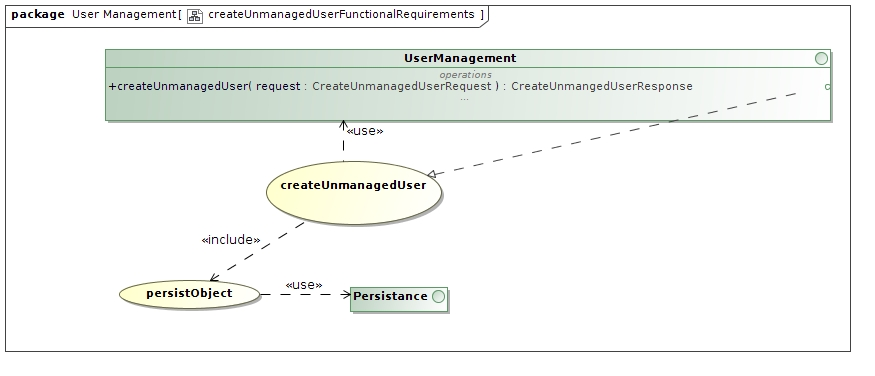
\includegraphics[scale=0.55]{../Diagrams and Charts/Users/createUnmanagedUserFunctionalRequirements.jpg}
		\caption{Functional Requirements for the createUnmanagedUser use case}
		\label{fig:CreateUnmanagedUserFR}
	\end{center}
\end{figure}

The only real lower level requirement is that a persistance interface is requiered
to access the database for object persistance.

\subsection{Update User}
Updates a users associated profile meta-data.

\subsubsection{Services Contract}
Figure \ref{fig:updateUserServicesContract} depicts the service contract for the \textbf{updateUser} service.

\begin{figure}[H]
  \begin{center}
  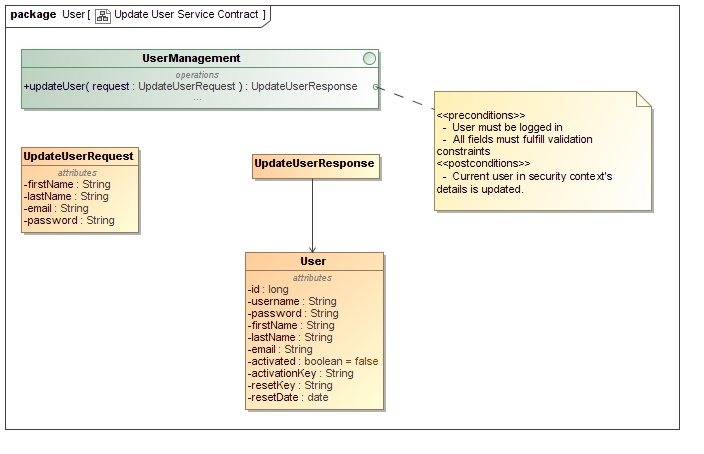
\includegraphics[scale=0.55]{../Diagrams and Charts/Users/Update User Service Contract.jpg}
  \caption{Service contract for the updateUser use case}
  \label{fig:updateUserServicesContract}
  \end{center}
\end{figure}

To update a user's profile the must hold true:
\begin{itemize}
	\item The user must change there own profile data or the user must be an admin user.
	\item The new data must subscribed to all validation requirements.
\end{itemize}

If the user is changing another user's profile data other than there own a \textbf{NotAuthorized} exception is thrown.  If the user is an admin user the request is regared as valid if all other requirements hold.

If the meta-data doesn't fulfill the required validation requirements, a \textbf{validationException} is thrown.

In addition, the service will be refused if the request does not comply to the data structure specification.

\subsubsection{Functional Requirements}
The lower level services required by the updateUser service to either check the
pre-conditions or address the post-conditions is shown in Figure \ref{fig:updateUserUseCase}.

\begin{figure}[H]
	\begin{center}
		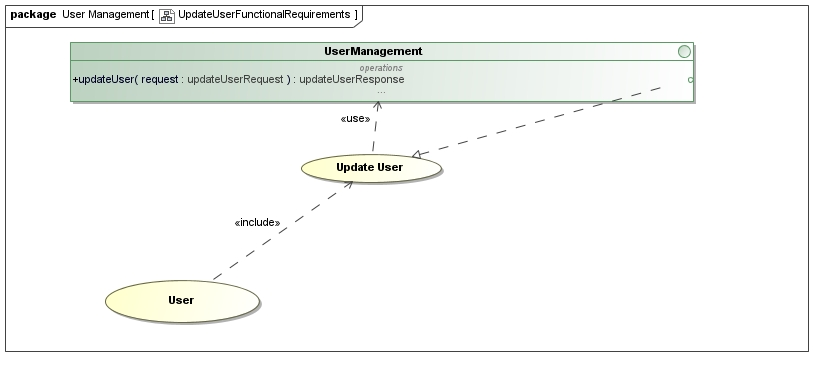
\includegraphics[scale=0.5]{../Diagrams and Charts/Users/UpdateUserFunctionalRequirements.jpg}
		\caption{The functional requirements for the updateUser use case}
		\label{fig:updateUserUseCase}
	\end{center}	
\end{figure}
\subsubsection{Process design}

\subsection{Get User With Authorities By ID}
Retrieves a user and their authorities by calling their ID

\subsubsection{Services Contract}
Figure \ref{fig:GetUserWithAuthoritiesByIDServicesContract} depicts the service contract for the \textbf{getUserWithAuthoritiesByID} service.

\begin{figure}[H]
	\begin{center}
		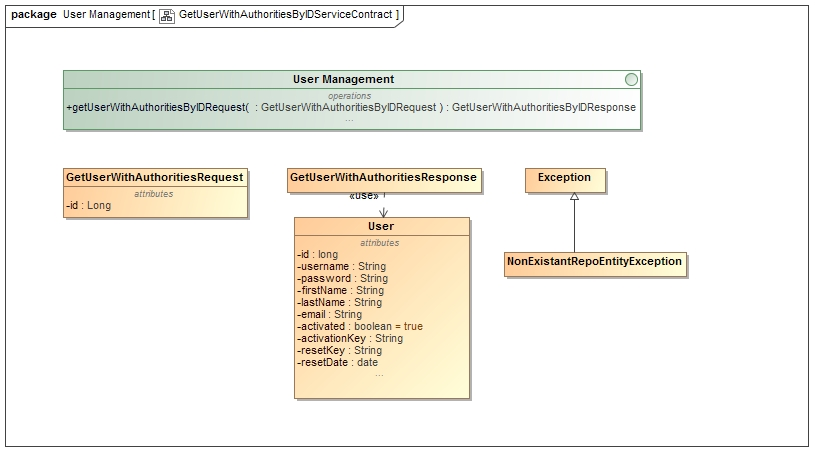
\includegraphics[scale=0.55]{../Diagrams and Charts/Users/Get User With Authorities By ID Service Contract.jpg}
		\caption{Service contract for the getUserWithAuthoritiesByID use case}
		\label{fig:GetUserWithAuthoritiesByIDServicesContract}
	\end{center}
\end{figure}

To get a user and their authorities by ID the following must hold true:
\begin{itemize}
	\item The user must exist in the current security context.
\end{itemize}

\subsubsection{Functional Requirements}
The lower level services required by the getUserWithAuthoritiesByID service to either check the
pre-conditions or address the post-conditions is shown in Figure \ref{fig:getUserWithAuthoritiesByIDUseCase}.

\begin{figure}[H]
	\begin{center}
		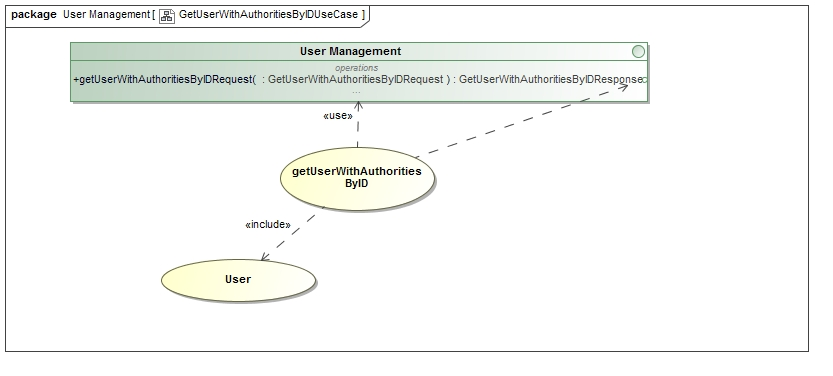
\includegraphics[scale=0.5]{../Diagrams and Charts/Users/Get User With Authorities By ID Use Case.jpg}
		\caption{The functional requirements for the getUserWithAuthoritiesByID use case}
		\label{fig:getUserWithAuthoritiesByIDUseCase}
	\end{center}	
\end{figure}

\subsection{Get User With Authorities By Login}
Retrieves a user and their authorities based on the username.

\subsubsection{Services Contract}
Figure \ref{fig:GetUserWithAuthoritiesByLoginServicesContract} depicts the service
contract for the \textbf{getUserWithAuthoritiesByLogin} service.

\begin{figure}[H]
	\begin{center}
		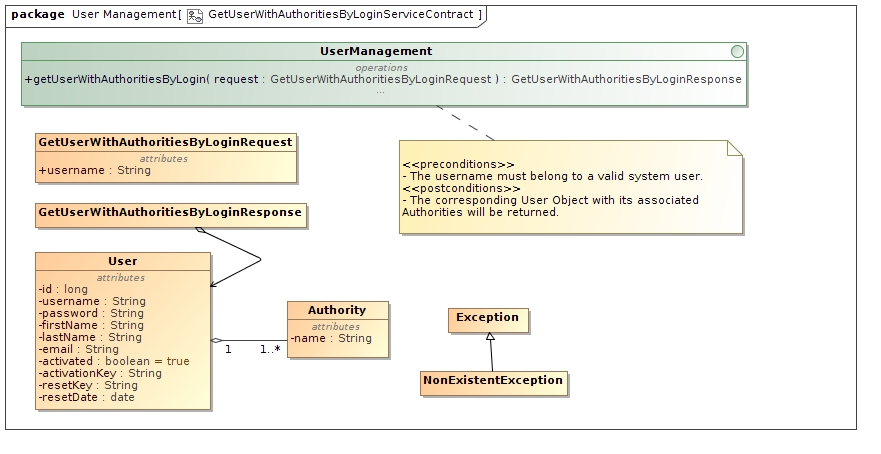
\includegraphics[scale=0.55]{../Diagrams and Charts/Users/GetUserWithAuthoritiesByLoginServiceContract.jpg}
		\caption{Service contract for the getUserWithAuthoritiesByLogin use case}
		\label{fig:GetUserWithAuthoritiesByLoginServicesContract}
	\end{center}
\end{figure}

To get a user and their authorities by ID the following must hold true:
\begin{itemize}
	\item The user must exist in the current security context.\\
	Otherwise a \textbf{NonExistentException} will be thrown.
\end{itemize}

\subsubsection{Functional Requirements}
The lower level services required by the getUserWithAuthoritiesByLogin service
to either check the pre-conditions or address the post-conditions is shown
in Figure \ref{getUserWithAuthoritiesByLoginFR}.

\begin{figure}[H]
	\begin{center}
		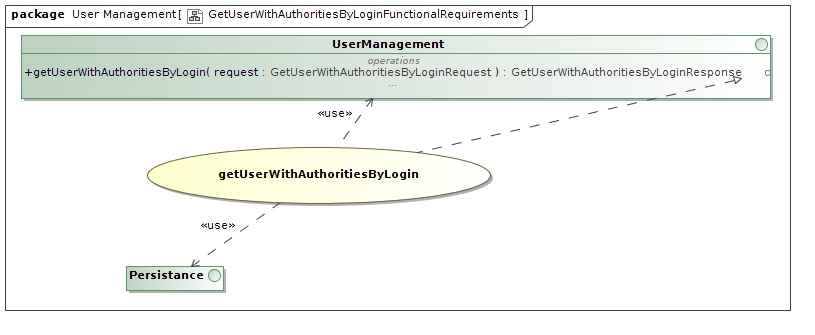
\includegraphics[scale=0.5]{../Diagrams and Charts/Users/GetUserWithAuthoritiesByLoginFunctionalRequirements.jpg}
		\caption{The functional requirements for the getUserWithAuthoritiesByLogin use case}
		\label{getUserWithAuthoritiesByLoginFR}
	\end{center}	
\end{figure}

In this case all that is required at a lower level is access to a persistance
interface to interact with the database.
%=================================================================================================================================

\subsection{Update User}
Updates the users details

\subsubsection{Services Contract}
Figure \ref{fig:updateUserServicesContract} depicts the service
contract for the \textbf{updateUser} service.

\begin{figure}[H]
	\begin{center}
		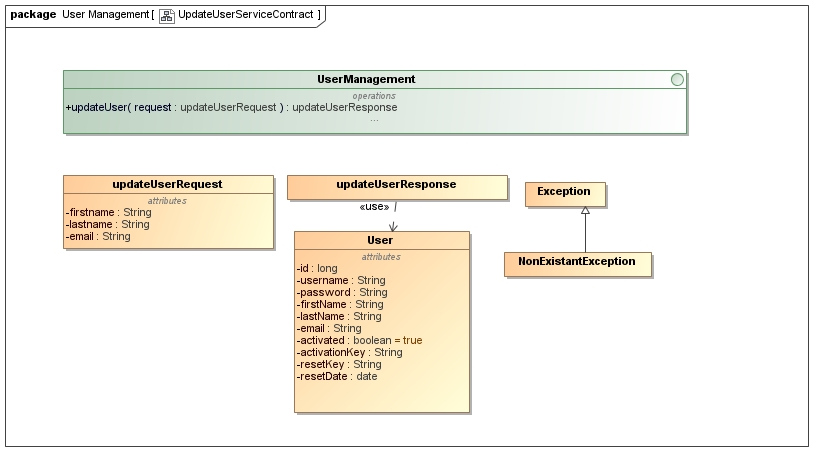
\includegraphics[scale=0.55]{../Diagrams and Charts/Users/UpdateUserServiceContract.jpg}
		\caption{Service contract for the updateUser use case}
		\label{fig:updateUserServicesContract}
	\end{center}
\end{figure}

To update the user the following must hold true:
\begin{itemize}
	\item The user must exist in the current security context.\\
	Otherwise a \textbf{NonExistentException} will be thrown.
	\item The details must be valid
\end{itemize}

\subsubsection{Functional Requirements}
The lower level services required by the updateUser service
to either check the pre-conditions or address the post-conditions is shown
in Figure \ref{fig:updateUserFR}.

\begin{figure}[H]
	\begin{center}
		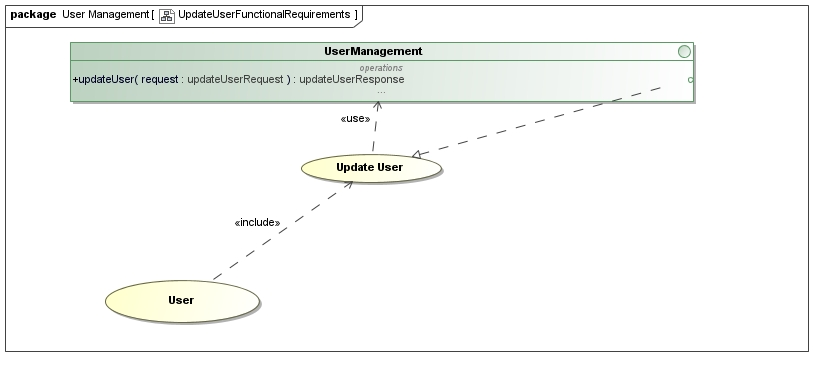
\includegraphics[scale=0.5]{../Diagrams and Charts/Users/UpdateUserFunctionalRequirements.jpg}
		\caption{The functional requirements for the updateUser use case}
		\label{fig:updateUserFR}
	\end{center}	
\end{figure}

In this case all that is required at a lower level is access to a persistance
interface to interact with the database.

\subsection{Delete User}
Deletes a specified user

\subsubsection{Services Contract}
Figure \ref{fig:DeleteUserSC} depicts the service
contract for the \textbf{deleteUser} service.

\begin{figure}[H]
	\begin{center}
		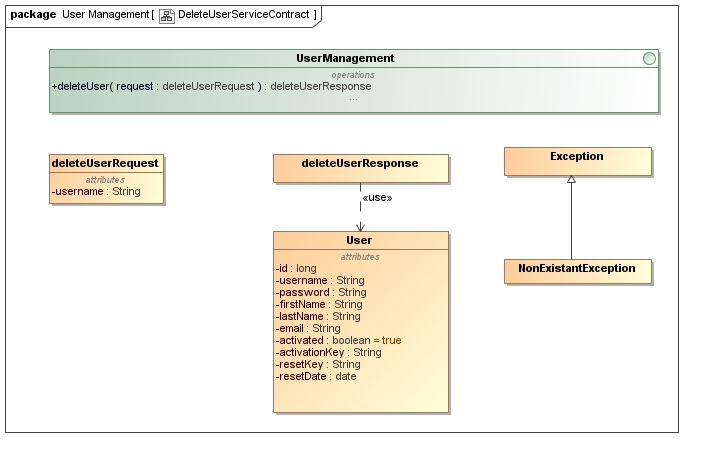
\includegraphics[scale=0.55]{../Diagrams and Charts/Users/DeleteUserServiceContract.jpg}
		\caption{Service contract for the deleteUser use case}
		\label{fig:DeleteUserSC}
	\end{center}
\end{figure}

To delete a user the following must hold true:
\begin{itemize}
	\item The user must exist in the current security context.\\
	Otherwise a \textbf{NonExistentException} will be thrown.
\end{itemize}

\subsubsection{Functional Requirements}
The lower level services required by the deleteUser service
to either check the pre-conditions or address the post-conditions is shown
in Figure \ref{fig:deleteUserFR}.

\begin{figure}[H]
	\begin{center}
		\includegraphics[scale=0.5]{../Diagrams and Charts/Users/deleteUserFunctionalRequirements.jpg}
		\caption{The functional requirements for the deleteUser use case}
		\label{fig:deleteUserFR}
	\end{center}	
\end{figure}

In this case all that is required at a lower level is access to a persistance
interface to interact with the database.


\subsection{Activate Registration}
Activates the registration of a user

\subsubsection{Services Contract}
Figure \ref{fig:activateRegSC} depicts the service
contract for the \textbf{activateRegistration} service.

\begin{figure}[H]
	\begin{center}
		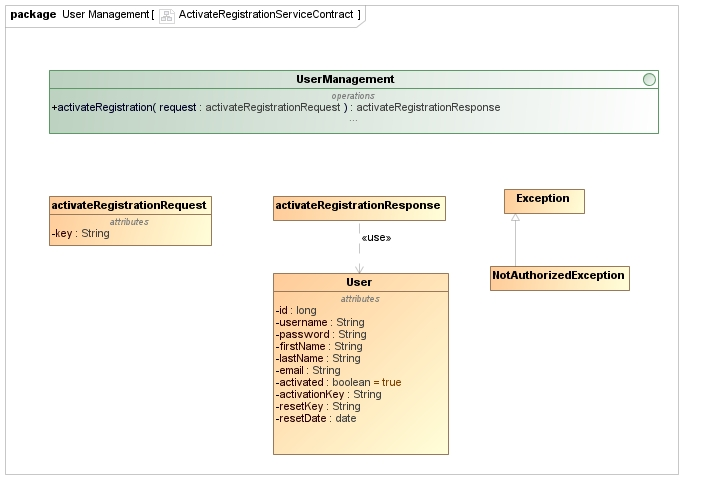
\includegraphics[scale=0.55]{../Diagrams and Charts/Users/ActivateRegistrationServiceContract.jpg}
		\caption{Service contract for the activateRegistration use case}
		\label{fig:activateRegSC}
	\end{center}
\end{figure}

To activate a registration following must hold true:
\begin{itemize}
	\item Key must be valid
\end{itemize}

\subsubsection{Functional Requirements}
The lower level services required by the activateRegistration service
to either check the pre-conditions or address the post-conditions is shown
in Figure \ref{fig:activateRegFR}.

\begin{figure}[H]
	\begin{center}
		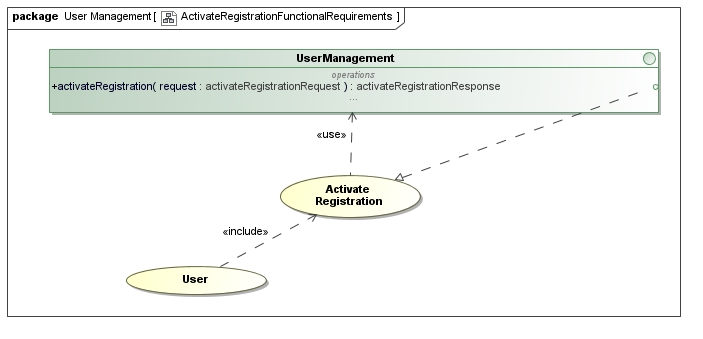
\includegraphics[scale=0.5]{../Diagrams and Charts/Users/ActivateRegistrationFunctionalRequirements.jpg}
		\caption{The functional requirements for the activateRegistration use case}
		\label{fig:activateRegFR}
	\end{center}	
\end{figure}

In this case all that is required at a lower level is access to a persistance
interface to interact with the database.


\subsection{Get User With Authorities}
Retrieves a user and their authorities.

\subsubsection{Services Contract}
Figure \ref{fig:GetUserWithAuthoritiesServicesContract} depicts the service
contract for the \textbf{getUserWithAuthorities} service.

\begin{figure}[H]
	\begin{center}
		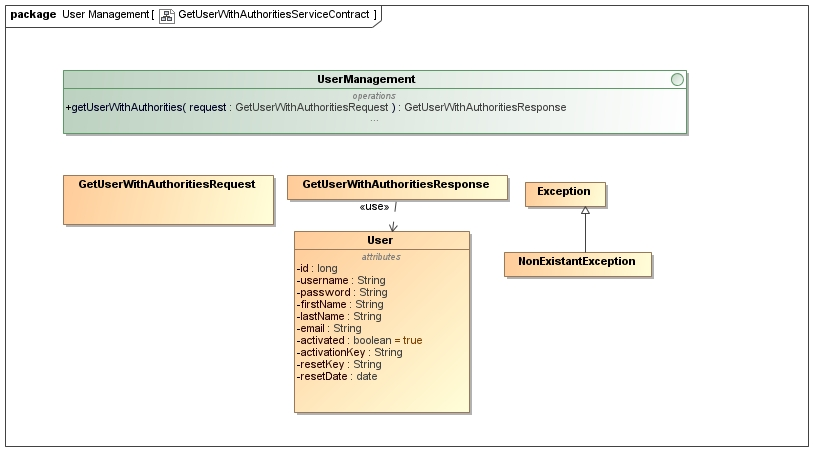
\includegraphics[scale=0.55]{../Diagrams and Charts/Users/GetUserWithAuthoritiesServiceContract.jpg}
		\caption{Service contract for the getUserWithAuthorities use case}
		\label{fig:GetUserWithAuthoritiesServicesContract}
	\end{center}
\end{figure}

To get a user and their authorities the following must hold true:
\begin{itemize}
	\item The user must exist in the current security context.\\
	Otherwise a \textbf{NonExistentException} will be thrown.
\end{itemize}

\subsubsection{Functional Requirements}
The lower level services required by the getUserWithAuthorities service
to either check the pre-conditions or address the post-conditions is shown
in Figure \ref{fig:getUserWithAuthoritiesFR}.

\begin{figure}[H]
	\begin{center}
		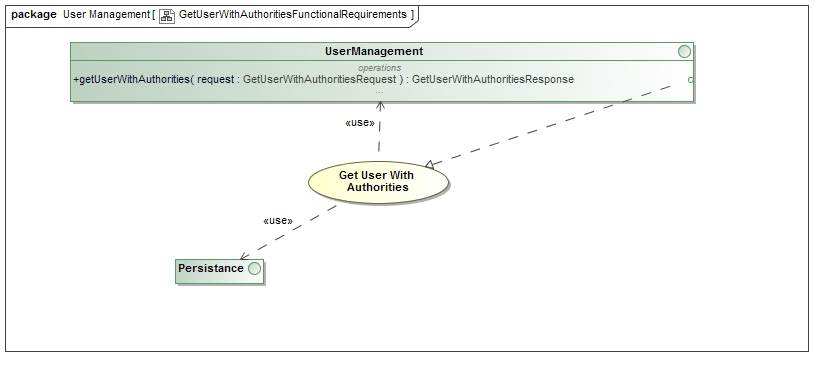
\includegraphics[scale=0.5]{../Diagrams and Charts/Users/GetUserWithAuthoritiesFunctionalRequirements.jpg}
		\caption{The functional requirements for the getUserWithAuthorities use case}
		\label{getUserWithAuthoritiesFR}
	\end{center}	
\end{figure}

In this case all that is required at a lower level is access to a persistance
interface to interact with the database.